\needspace{15\baselineskip}% room for the wrapped icon (it cannot break across pages)
\subsection{Iron-air battery, 100~h (75~\$/kWh)}\label{sec:iron-air}
\techicon{iron-air}{An iron-air enclosure, opened: cells with iron pellets, air drawn in from the roof.}
Iron-air batteries (Figure~\ref{fig:icon-iron-air}) rust iron with oxygen from the air when they discharge and turn the rust back into iron when they charge.
Iron is cheap, which gives them a low energy cost and makes them suitable for long-duration storage.
However, they are at the start of commercial deployment, so their cost remains uncertain and no learning trend has been observed yet.

The CAPEX of 75~\$/kWh is the price before subsidies for a system with a fixed 100~hours of storage.
It was inferred from the only project with disclosed costs, Form Energy's 300~MW / 30~GWh system at Pine Island, for which Google paid about 1~bn~USD \citep{techcrunch2026}.
That is about 32~\$/kWh after US tax credits and other incentives; adding these back gives about 2.3~bn~USD, or 75~\$/kWh in 2024 dollars \citep{weaver2026} (Figure~\ref{fig:iron-air}).

\begin{figure}[htbp]\centering
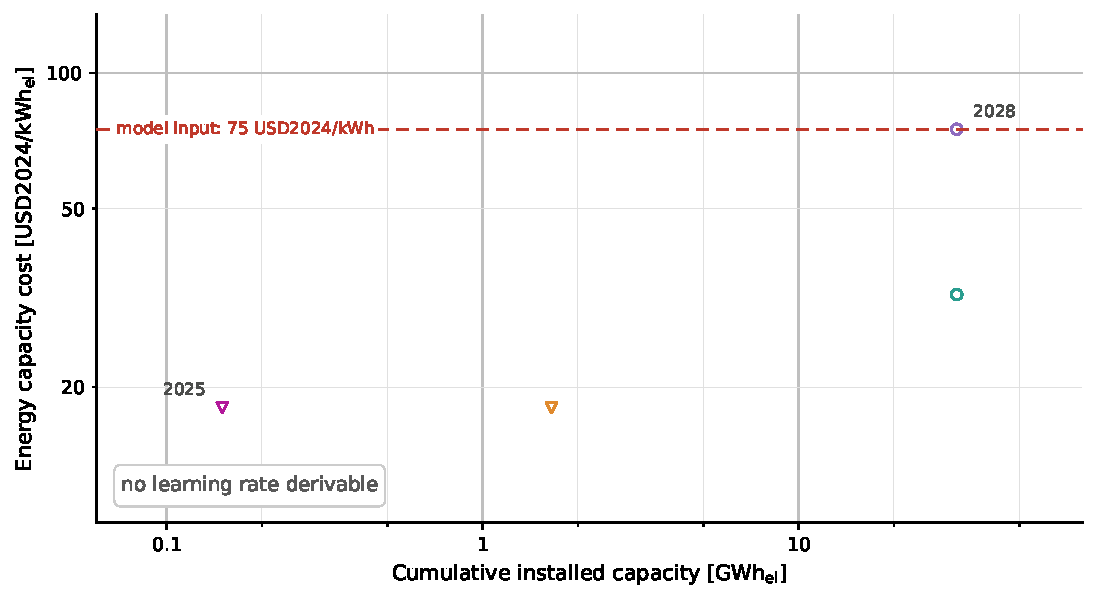
\includegraphics[width=\textwidth]{../../../misc-quarter1/technology-costs/figures/learning/iron-air.pdf}
\caption{
  Iron-air battery cost per kWh against cumulative capacity.
  Triangles: Form's cost target from its modelling recommendations [1] and vendor target [2] \citep{form2023}.
  Circles: Pine Island after incentives [3] \citep{techcrunch2026} and before incentives [4] \citep{weaver2026}.
  Dashed red line: the model input.
}\label{fig:iron-air}
\end{figure}

The learning rate is 15\,\% on the energy part.
There is no cost history yet, so we use a literature value of $15\pm5$\,\% \citep{riepin2025}.
At this rate, reaching Form's target of 15--20~\$/kWh \citep{form2023} takes eight to ten doublings of cumulative capacity.

The efficiency of 0.41 is the product of 0.70 for charging and 0.59 for discharging, and the fixed O\&M is 1\,\% per year of a 35~\$/kWh system, both from Form's modelling recommendations \citep{form2023}.
Existing capacity is Great River Energy's 1.5~MW / 150~MWh pilot in Cambridge, Minnesota; further projects are under construction or planned at Pine Island and in Georgia and Maine.
The lead time is 1.5~years.
